\documentclass{article}
\usepackage{fancyhdr}
\usepackage{ctex}
\usepackage{listings}
\usepackage{graphicx}
\usepackage[a4paper, body={18cm,22cm}]{geometry}
\usepackage{amsmath,amssymb,amstext,wasysym,enumerate,graphicx}
\usepackage{float,abstract,booktabs,indentfirst,amsmath}
\usepackage{array}
\usepackage{booktabs}
\usepackage{multirow}
\usepackage{url}
\usepackage{diagbox}
\renewcommand\arraystretch{1.4}
\usepackage{indentfirst}
\setlength{\parindent}{2em}
\usepackage{enumerate}
\setmonofont{MesloLGS NF}
\usepackage{listings}
\usepackage{xcolor}
\usepackage{makecell}
\setCJKmonofont{黑体}
\lstset{
    language = [x86masm]Assembler,
    xleftmargin = 3em,xrightmargin = 3em, aboveskip = 1em,
	backgroundcolor = \color{white}, % 背景色
	basicstyle = \small\ttfamily, % 基本样式 + 小号字体
	rulesepcolor= \color{gray}, % 代码块边框颜色
	breaklines = true, % 代码过长则换行
	numbers = left, % 行号在左侧显示
	numberstyle = \small, % 行号字体
    numbersep = -14pt, 
	keywordstyle = \color{blue!50!red!100}, % 关键字颜色
	commentstyle =\color{red!50!green!50!blue!60}, % 注释颜色
	stringstyle = \color{red}, % 字符串颜色
	frame = shadowbox, % 用(带影子效果)方框框住代码块
	showspaces = false, % 不显示空格
	columns = fixed, % 字间距固定
} 
%--------------------页眉--------------------%
\pagestyle{fancy}
\fancyhead[L]{}
\fancyhead[R]{}
\fancyhead[C]{华东师范大学软件工程学院实验报告}
\fancyfoot[C]{-\thepage-}
\renewcommand{\headrulewidth}{1.5pt}
%--------------------标题--------------------%
\begin{document}
\begin{center}
  \LARGE{{\textbf{\heiti 华东师范大学软件工程学院实验报告}}}
  \begin{table}[H]
    \centering
    \begin{tabular}{p{2cm}p{4cm}<{\centering}p{1cm}p{2cm}p{6cm}<{\centering}}
      姓\qquad 名: & 李鹏达 & \quad & 学\qquad 号: & 10225101460                  \\ \cline{2-2} \cline{5-5}
      实验编号:    & Lab 03 & \quad & 实验名称:    & {Building A Cache Simulator}
      \\ \cline{2-2} \cline{5-5}
    \end{tabular}
  \end{table}
\end{center}
\rule{\textwidth}{1pt}
%--------------------正文--------------------%
\section{实验目的}
\large
\begin{enumerate}[1)]
  \item 深入了解高速缓存的原理与结构
  \item 学习通过利用高速缓存的结构优化效率
\end{enumerate}
\normalsize
\section{实验内容与实验步骤}
\subsection{实验内容}
\large
本练习将帮助您了解缓存内存对 C 语言性能的影响
程序。

实验室由两部分组成。在第一部分中,您将编写一个小的 C 程序(大约 200-300 行)

模拟高速缓存的行为。在第二部分中,您将优化一个小矩阵转置
函数,目的是最大限度地减少缓存未命中次数。

\subsubsection{Part A:Writing a Cache Simulator}
在 A 部分中,您将在 csim.c 中编写一个缓存模拟器,该模拟器将 valgrind 内存跟踪作为输入,
模拟此跟踪上缓存的命中/未命中行为,并输出命中,
未命中和替换总数。

我们先对原理进行分析。
在输入中会提供高速缓存的$s$、$E$、$b$,从而确定该高速缓存有$S=2^s$组,每组中有E行,每行的高速缓存块大小为$B=2^b$字节,通过malloc函数进行动态内存分配即可构造出模拟的高速缓存。
依据存储器层次结构,来模拟高速缓存块映射的命中、不命中以及替换过程,替换策略为LRU(最近最少使用)。

首先,我们先定义行结构体和所需的全局变量。
\begin{lstlisting}[xleftmargin = 4em,xrightmargin = 4em, aboveskip = 1em, numbers = left, language = C]
    typedef struct {
        int valid; // valid
        long tag;  // tag
        long time; // time
    } line;

    line** cache;

    int hits = 0;
    int misses = 0;
    int evictions = 0;

    int s, E, b;
    char trace_file[1000];
    int verbose = 0; // false
\end{lstlisting}

接下来,我们需要在main函数中对命令行输入的参数进行解析。

getopt 是一个在 UNIX 类操作系统中常用的库函数,它用于解析命令行参数。该函数会返回在命令行中找到的选项字符,如果选项需要一个参数,那么 optarg 全局变量就会被设置为该参数。

函数通过字符串 "hvs:E:b:t:" 定义了可以接受的命令行选项。在这个字符串中,如果选项后面有冒号,那么它就需要一个参数。

处理每个选项:函数使用了一个 switch 语句来处理找到的每个选项。case 'h' 是显示帮助信息,case 'v' 是决定是否输出详细信息,case 's'、'E' 和 'b' 是设置缓存参数,case 't' 指定输入文件。

如果 getopt 找到了一个未知的选项,那么函数会显示使用说明,并退出程序。这个行为可以帮助用户了解如何正确使用程序。

总的来说编写思路是:使用 getopt 函数解析命令行参数,并针对每个可接受的选项进行处理。如果遇到了未知的选项,就显示使用说明并退出程序。

\begin{lstlisting}[xleftmargin = 4em,xrightmargin = 4em, aboveskip = 1em, numbers = left, language = C]
    char opt;
    const char* usage = "usage: ./csim-ref [-hv] -s <s> -E <E> -b <b> -t <tracefile>";
    while ((opt = getopt(argc, argv, "hvs:E:b:t:")) != EOF) {
        switch (opt) {
            case 'h':
                fprintf(stdout, "%s", usage);
                exit(0);
                break;
            case 'v':
                verbose = 1;
                break;
            case 's':
                s = atoi(optarg);
                break;
            case 'E':
                E = atoi(optarg);
                break;
            case 'b':
                b = atoi(optarg);
                break;
            case 't':
                strcpy(trace_file, optarg);
                break;
            default:
                fprintf(stdout, "%s", usage);
                exit(-1);
                break;
        }
    }
\end{lstlisting}

接下来,我们需要对高速缓存进行初始化.我们首先计算$S = 2 ^ s$,然后使用malloc函数动态分配内存。

\begin{lstlisting}[xleftmargin = 4em,xrightmargin = 4em, aboveskip = 1em, numbers = left, language = C]
    void init() {
        int S = 1 << s; // 2 ^ s
        cache = (line**)malloc(sizeof(line*) * S);
        for (int i = 0; i < S; i++) {
            cache[i] = (line*)malloc(sizeof(line) * E);
            for (int j = 0; j < E; j++) {
                cache[i][j].valid = 0;
                cache[i][j].tag = -1;
                cache[i][j].time = 0;
            }
        }
    }
\end{lstlisting}

然后,我们需要读取处理文件中的命令。

处理输入文件:接着,函数开始读取输入文件。对于文件中的每一行,函数首先判断是否是 'I' 开头,如果是,就忽略这一行。否则,函数就解析这一行,得到操作类型('S'、'L' 或 'M'),地址和大小。然后,根据操作类型,函数调用 update 函数模拟一次 CPU 访问缓存的过程。

处理详细输出:在每次调用 update 之后,如果 verbose 变量被设置为 1,那么函数就会输出一些详细信息,包括操作类型、地址、大小,以及这次访问的结果(命中、未命中或替换)。

释放内存和关闭文件:在处理完输入文件的所有行之后,释放了申请的内存,关闭输入文件。

\begin{lstlisting}[xleftmargin = 4em,xrightmargin = 4em, aboveskip = 1em, numbers = left, language = C]
    void get_trace() {
        char operation;
        unsigned long address;
        int size;
        FILE* fp = fopen(trace_file, "r");
        if (fp == NULL) exit(-1);
        while (fscanf(fp, " %c %lx,%d\n", &operation, &address, &size) > 0) {

            // do operation
            switch (operation) {
                case 'L':
                    update(address, operation, size);
                    break;
                case 'S':
                    update(address, operation, size);
                    break;
                case 'M':
                    update(address, operation, size);
                    update(address, operation, size);
                    break;
            }

            // update time
            for (int i = 0; i < (1 << s); i++) {
                for (int j = 0; j < E; j++) {
                    if (cache[i][j].valid) {
                        cache[i][j].time++;
                    }
                }
            }
        }
        fclose(fp);
    }

    void free_cache() {
        for (int i = 0; i < (1 << s); i++) {
            free(cache[i]);
        }
        free(cache);
    }
\end{lstlisting}

接下来,我们应该具体模拟高速缓存的工作过程。

update 函数的目的是模拟 CPU 访问缓存的过程。给定一个内存地址,这个函数会在缓存中查找对应的行,然后根据查找结果更新命中次数(hits)、未命中次数(misses)和替换次数(evictions)。以下是实现这个目的的详细步骤:

计算标签和集合索引:首先,函数计算了给定地址的标签(tag)和集合索引(set)。这是通过移位操作和位掩码完成的。对于给定的内存地址,标签是地址的高位部分,集合索引是地址的中间部分。这些部分的大小由缓存的参数决定。

访问对应的缓存集合:然后,函数访问了缓存中对应的集合。这个集合是一个 line 结构体的数组,每个元素代表一行。

在集合中查找标签:接着,函数在集合中查找标签。如果找到了对应的标签,那么就发生了一次命中,函数就会增加命中次数,并更新对应行的时间戳。

处理未命中的情况:如果在集合中没有找到标签,那么就发生了一次未命中。此时,函数会查找一个空行或者使用 LRU 策略找到一个要被替换的行。如果找到了空行,那么就将新标签放入这个行;如果所有的行都不为空,那么就替换最久未使用的行。在这个过程中,函数可能会增加未命中次数和替换次数。

通过这些步骤,update 函数实现了 CPU 访问缓存的模拟。这个函数的实现思路是基于缓存的工作原理和 LRU 替换策略的。

\begin{lstlisting}[ xleftmargin = 4em,xrightmargin = 4em, aboveskip = 1em, numbers = left, language = C]
    void update(unsigned long address, char operation, int size) {
        int set = (address >> b) & ((-1U) >> (64 - s));
        int tag = address >> (b + s);
    
        // hit
        for (int i = 0; i < E; i++) {
            if (cache[set][i].tag == tag) {
                cache[set][i].time = 0;
                hits++;
                if (verbose) {
                    printf("%c %lx,%d hit\n", operation, address, size);
                }
                return;
            }
        }
    
        // miss
        for (int i = 0; i < E; i++) {
            if (cache[set][i].valid == 0) {
                cache[set][i].valid = 1;
                cache[set][i].tag = tag;
                cache[set][i].time = 0;
                misses++;
                if (verbose) {
                    printf("%c %lx,%d miss\n", operation, address, size);
                }
                return;
            }
        }
    
        // miss eviction
        evictions++;
        misses++;
        int max_time = -1;
        int max_time_index = -1;
        for (int i = 0; i < E; i++) {
            if (cache[set][i].time > max_time) {
                max_time = cache[set][i].time;
                max_time_index = i;
            }
        }
        cache[set][max_time_index].tag = tag;
        cache[set][max_time_index].time = 0;
        if (verbose) {
            printf("%c %lx,%d miss eviction\n", operation, address, size);
        }
    }
\end{lstlisting}

这样,我们便完成了模拟高速缓存的全部过程。

\subsubsection{Part B: Optimizing Matrix Transpose}

在 B 部分中,您将在 trans.c 中编写一个转置函数,该函数会导致尽可能少的缓存未命中。

\paragraph*{1)$32 \times 32$}
在本部分,我们需要转置一个$32 \times 32$的矩阵。

因为一行有32个bytes,也就是能一次保存8个int,我们可以将矩阵拆分成多个$8 \times 8$分块矩阵来进行转置。那么可以得到代码如下:

\begin{lstlisting}[xleftmargin = 4em,xrightmargin = 4em, aboveskip = 1em, numbers = left, language = C]
    for (int i = 0; i < 32; i += 8) {
        for (int j = 0; j < 32; j += 8) {
            for (int k = i; k < (i + 8); k++) {
                int temp1, temp2, temp3, temp4, temp5, temp6, temp7, temp8;
                temp1 = A[k][j];
                temp2 = A[k][j + 1];
                temp3 = A[k][j + 2];
                temp4 = A[k][j + 3];
                temp5 = A[k][j + 4];
                temp6 = A[k][j + 5];
                temp7 = A[k][j + 6];
                temp8 = A[k][j + 7];
                B[j][k] = temp1;
                B[j + 1][k] = temp2;
                B[j + 2][k] = temp3;
                B[j + 3][k] = temp4;
                B[j + 4][k] = temp5;
                B[j + 5][k] = temp6;
                B[j + 6][k] = temp7;
                B[j + 7][k] = temp8;
            }
        }
    }
\end{lstlisting}

\paragraph*{2)$64 \times 64$}
在本部分,我们需要转置一个$64 \times 64$的矩阵。

我们可以通过将矩阵先进行8划分,再进行4划分,由于我们通过4划分后的分块矩阵进行多次转置操作,实现整个矩阵的转置。

首先,我们将每个$8 \times 8$的大块中上面的两个$4 \times 4$小块进行内部转置。
然后,还需要将下面两个小块进行内部转置。
最后,需要对$8 \times 8$的大块中左下角和右上角两个块进行转置。
代码如下:

\begin{lstlisting}[xleftmargin = 4em,xrightmargin = 4em, aboveskip = 1em, numbers = left, language = C]
    for (int i = 0; i < N; i += 8) {
        for (int j = 0; j < M; j += 8) {
            int temp1, temp2, temp3, temp4, temp5, temp6, temp7, temp8;
            for (int k = i; k < i + 4; k++) {
                temp1 = A[k][j];
                temp2 = A[k][j + 1];
                temp3 = A[k][j + 2];
                temp4 = A[k][j + 3];
                temp5 = A[k][j + 4];
                temp6 = A[k][j + 5];
                temp7 = A[k][j + 6];
                temp8 = A[k][j + 7];

                B[j][k] = temp1;
                B[j + 1][k] = temp2;
                B[j + 2][k] = temp3;
                B[j + 3][k] = temp4;
                B[j][k + 4] = temp5;
                B[j + 1][k + 4] = temp6;
                B[j + 2][k + 4] = temp7;
                B[j + 3][k + 4] = temp8;
            }
            for (int k = j; k < j + 4; k++) {
                temp1 = A[i + 4][k];
                temp2 = A[i + 5][k];
                temp3 = A[i + 6][k];
                temp4 = A[i + 7][k];
                temp5 = B[k][i + 4];
                temp6 = B[k][i + 5];
                temp7 = B[k][i + 6];
                temp8 = B[k][i + 7];

                B[k][i + 4] = temp1;
                B[k][i + 5] = temp2;
                B[k][i + 6] = temp3;
                B[k][i + 7] = temp4;
                B[k + 4][i] = temp5;
                B[k + 4][i + 1] = temp6;
                B[k + 4][i + 2] = temp7;
                B[k + 4][i + 3] = temp8;
            }
            for (int k = i + 4; k < i + 8; k++) {
                temp1 = A[k][j + 4];
                temp2 = A[k][j + 5];
                temp3 = A[k][j + 6];
                temp4 = A[k][j + 7];

                B[j + 4][k] = temp1;
                B[j + 5][k] = temp2;
                B[j + 6][k] = temp3;
                B[j + 7][k] = temp4;
            }
        }
}
\end{lstlisting}

\paragraph*{1)$61 \times 67$}
在本部分,我们需要转置一个$61 \times 67$的矩阵。

考虑分成$4\times 17$的矩阵。代码如下:

\begin{lstlisting}[xleftmargin = 4em,xrightmargin = 4em, aboveskip = 1em, numbers = left, language = C]
    for (int i = 0; i < 67; i += 17) {
        for (int j = 0; j < 61; j += 4) {
            for (int k = i; k < (i + 17 > 67 ? 67 : i + 17); k++) {
                for (int l = j; l < (j + 4 > 61 ? 61 : j + 4); l++) {
                    B[l][k] = A[k][l];
                }
            }
        }
    }
\end{lstlisting}

\normalsize
\subsection{实验步骤}
\large
\begin{enumerate}[1)]
  \item 解打包cachelab-handout.tar
        \begin{lstlisting}[language=bash]
    linux> tar -xvf cachelab-handout.tar
    \end{lstlisting}
  \item 阅读要求,编写csim.c和trans.C
  \item 编译
        \begin{lstlisting}[language=bash]
    linux> make
    \end{lstlisting}
  \item 评测
        \begin{lstlisting}[language=bash]
    linux> ./driver.py
    \end{lstlisting}

\end{enumerate}
\normalsize
\section{实验过程与分析}
\large

实验的运行结果如下:
\begin{figure}[H]
  \centering
  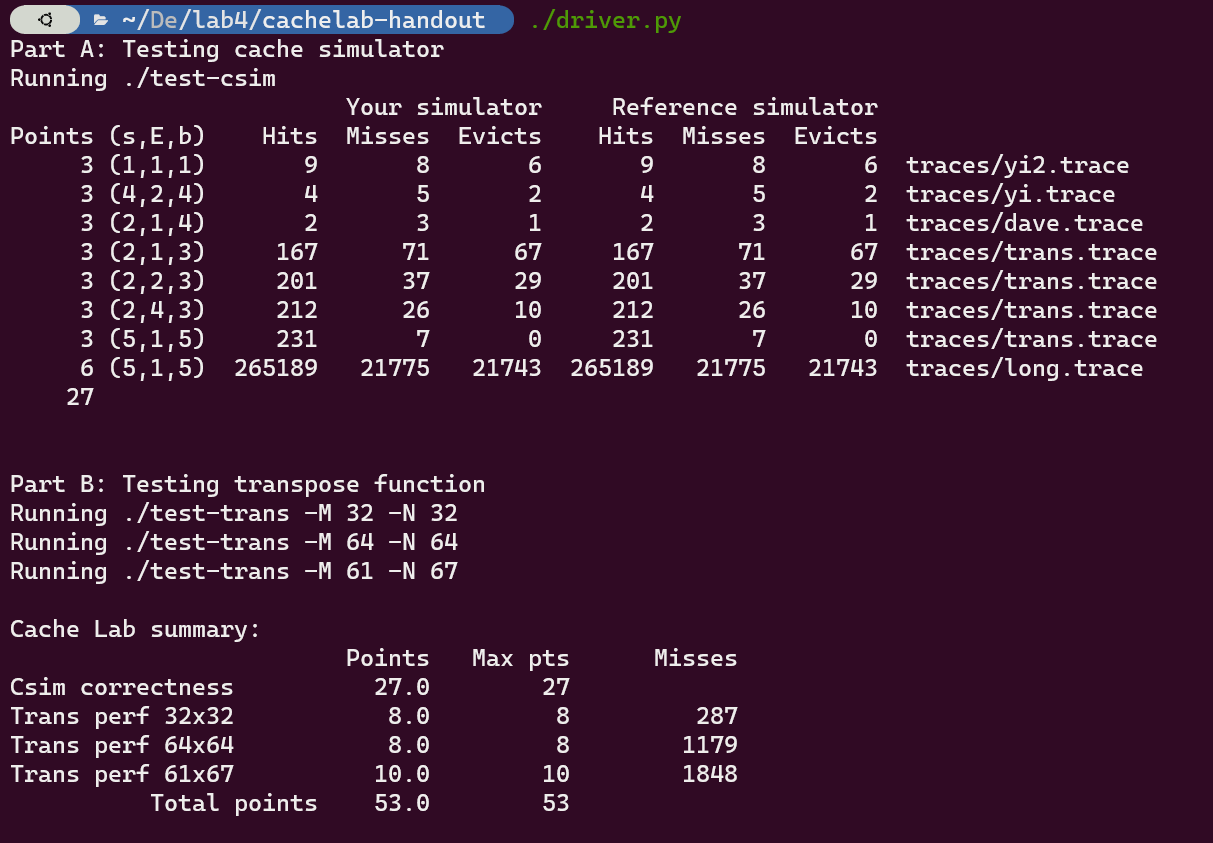
\includegraphics[width=15cm]{1.png}
  \caption{运行结果}
\end{figure}


\normalsize
\section{实验结果总结}
\large
在本次实验中,我学习到了高速缓存的基本结构,同时也学会了利用高速缓存的结构优化效率。

\normalsize
\large




\normalsize
\end{document}